\documentclass[10pt,letterpaper]{article}
\usepackage[top=0.85in,left=2.75in,footskip=0.75in]{geometry}


\usepackage{currfile}
\lefthyphenmin=3
\righthyphenmin=2

\usepackage{url}
\usepackage{graphicx,epsfig,verbatim,enumerate}
\usepackage{amssymb,amsmath}

\usepackage{xcolor}
\usepackage{color}
\newcommand{\todo}[1]{\noindent\textcolor{red}{{$\Box$ #1}}}
\definecolor{lightgrey}{rgb}{0.5,0.5,0.5}

\usepackage{rotating}
\usepackage{longtable}
\usepackage{array}

\usepackage{listings,color,setspace}

\newcommand{\avg}[1]{\left\langle#1\right\rangle}
\newcommand{\tavg}[1]{\langle#1\rangle}

\newcommand{\LavgHa}[2]{\tavg{L_{#1,#2}}}
\newcommand{\LavgHaN}[2]{\tavg{L_{#1,#2}}}
\newcommand{\Lavg}{\tavg{L}}

\newcommand{\sindex}[1]{}
\newcommand{\nindex}[1]{}

\newcommand{\etal}{\textit{et al.}}
\newcommand{\www}[1]{\url{#1}}
\newcommand{\req}[1]{(\ref{#1})}
\newcommand{\Req}[1]{Eq.~(\ref{#1})}

\newcommand{\yes}{}
\newcommand{\no}{}
\newcommand{\tbf}{\textbf}
\newcommand{\tit}{\textit}

\newcommand{\dee}[1]{\mbox{d}#1}
\newcommand{\pdiff}[2]{\frac{\partial #1}{\partial #2}}
\newcommand{\partialdiff}[2]{\frac{\partial #1}{\partial #2}}
\newcommand{\pdiffsq}[2]{\frac{\partial^2 #1}{{\partial #2}^2}}
\newcommand{\diff}[2]{\frac{{\rm d}#1}{{\rm d}#2}}
\newcommand{\diffsq}[2]{\frac{{\rm d}^{2}#1}{{\rm d} {#2}^2}}
\newcommand{\tdiff}[2]{\mbox{d} #1/\mbox{d} #2}
\newcommand{\tdiffsq}[2]{\mbox{d}^{2} #1/\mbox{d} {#2}^2}
\newcommand{\tpdiff}[2]{\partial #1/\partial #2}
\newcommand{\tpdiffsq}[2]{\partial^2 #1/\partial {#2}^2}
\newcommand{\postdee}[1]{\,\mbox{d}#1}
\newcommand{\rhoref}{\rho_{\text{ref}}}
\newcommand{\dphi}{\text{d}\phi}

\newcommand{\mbe}{\mathbf{\epsilon}}
\newcommand{\mbx}{\mathbf{x}}
\newcommand{\mby}{\mathbf{y}}
\newcommand{\mbd}{\mathbf{d}}
\newcommand{\mbB}{\mathbf{B}}
\newcommand{\mbW}{\mathbf{W}}
\newcommand{\mbR}{\mathbf{R}}
\newcommand{\mbH}{\mathbf{H}}
\newcommand{\mbK}{\mathbf{K}}
\newcommand{\mbP}{\mathbf{P}}
\newcommand{\mbZ}{\mathbf{Z}}
\newcommand{\mbw}{\mathbf{w}}
\newcommand{\mbX}{\mathbf{X}}
\newcommand{\mbY}{\mathbf{Y}}
\newcommand{\mb}{\mathbf{}}
\newcommand{\expv}[1]{E \left [ #1 \right ]}

\newcommand{\PreserveBackslash}[1]{\let\temp=\\#1\let\\=\temp}
\newcommand{\PBS}[1]{\let\temp=\\#1\let\\=\temp}

\newcommand{\kstar}{d^\ast}
\newcommand{\kstari}{d_i^\ast}

\newcommand{\dstar}{d^\ast}
\newcommand{\dstari}{d_i^\ast}

\newcommand{\phifix}{{\phi^{\ast}}}
\newcommand{\phifixc}{{\phi_c^{\ast}}}
\newcommand{\phifixb}{{\phi_b^{\ast}}}

\newcommand{\Gfun}{G}

\newcommand{\dstardist}{g}
\newcommand{\dosedist}{f}
\newcommand{\dosedistk}{f^{k\star}}

\newcommand{\meandegree}{z}
\newcommand{\kmax}{k_{\rm max}}

\newcommand{\wff}{\url{wefeelfine.org}}

\newcommand{\fplus}{f_{+}}
\newcommand{\fminus}{f_{-}}
\newcommand{\aplus}{a_{+}}
\newcommand{\aminus}{a_{-}}

\newcommand{\havg}[1]{h_{\rm avg}(#1)}
\newcommand{\havgword}[1]{h_{\rm avg}(\mbox{`#1'})}
\newcommand{\havgsup}[1]{h_{\rm avg}^{#1}}
\newcommand{\havgsuparg}[2]{h_{\rm avg}^{#1}(#2)}
\newcommand{\havgfn}{h_{\rm avg}}
\newcommand{\havgfnamb}{h_{\rm avg}^{\rm (amb)}}
\newcommand{\havgfnnorm}{h_{\rm avg}^{\rm (norm)}}

\newcommand{\pinstA}{\rm inst}
\newcommand{\pinstB}{j}

\newcommand{\popA}{\rm inst}
\newcommand{\popB}{\rm pop}



\usepackage{changepage}

\usepackage[utf8]{inputenc}

\usepackage{textcomp,marvosym}

\usepackage{fixltx2e}

\usepackage{amsmath,amssymb}

\usepackage{cite}

\usepackage{hyperref}

\usepackage[right]{lineno}

\usepackage{microtype}
\DisableLigatures[f]{encoding = *, family = * }

\usepackage{rotating}


\raggedright
\setlength{\parindent}{0.5cm}
\textwidth 5.25in 
\textheight 8.75in

\usepackage[aboveskip=1pt,labelfont=bf,labelsep=period,justification=raggedright,singlelinecheck=off]{caption}

\bibliographystyle{plos-style}

\makeatletter
\renewcommand{\@biblabel}[1]{\quad#1.}
\makeatother

\date{}

\usepackage{lastpage,fancyhdr,graphicx}
\usepackage{epstopdf}
\pagestyle{myheadings}
\pagestyle{fancy}
\fancyhf{}
\lhead{
\includegraphics[width=2.0in]{fig0_PLOS-submission.pdf}}

\rfoot{\thepage/13}
\renewcommand{\footrule}{\hrule height 2pt \vspace{2mm}}
\fancyheadoffset[L]{2.25in}
\fancyfootoffset[L]{2.25in}
\lfoot{\sf PLOS}



\newcommand{\lorem}{{\bf LOREM}}
\newcommand{\ipsum}{{\bf IPSUM}}




\begin{document}

\section*{Supporting Information}

\newwrite\tempfile
\immediate\openout\tempfile=startsupp-plos.txt
\immediate\write\tempfile{\thepage}
\immediate\closeout\tempfile

\rfoot{\thepage/S12}
\setcounter{page}{1}
\renewcommand{\thepage}{S\arabic{page}}
\renewcommand{\theequation}{S\arabic{equation}}
\renewcommand{\thefigure}{S\arabic{figure}}
\renewcommand{\thetable}{S\arabic{table}}
\setcounter{figure}{0}
\setcounter{table}{0}

\subsection*{S1 Appendix: Computational Details and Explicit Equations Used}
\label{S1}

In this section, we first present the governing equations for the flow in our thermal convection loop experiment.
A spatial and temporal discretization of the governing equations is then necessary so that they may be solved numerically.
After discretization, we must specify the boundary conditions.
With the mesh and boundary conditions in place, we can then simulate the flow with a computational fluid dynamics solver.

We now discuss the equations, mesh, boundary conditions, and solver in more detail.
With these considerations, we present our simulations of the thermosyphon.
For a complete derivation of the equations used, see \cite{reagan2013}.

We consider the incompressible Navier-Stokes equations with the Boussinesq approximation to model the flow of water inside a thermal convection loop.
Here we present the main equations that are solved numerically, noting the assumptions that are necessary in their derivation.
In standard notation, for $u,v,w$ the velocity in the $x,y,z$ direction, respectively, the continuity equation for an incompressible fluid is
\begin{equation} \frac{\partial u}{\partial x} + \frac{\partial v}{\partial y} + \frac{\partial w}{\partial z} = 0. \label{eq:NScontIco} \end{equation}

The momentum equations, in tensor notation with bars representing averaged quantities (long timesteps are used, requiring integration), are
\begin{equation} \rho_\text{ref} \left ( \frac{\partial \bar{u}_i}{\partial t} + \frac{\partial}{\partial x_j} \left( \bar{u}_j \bar{u}_i \right) \right )
= -\frac{\partial \bar{p}} {\partial{x_i}} +  \mu \frac{\partial \bar{u}_i}{\partial x_j^2} + \rhoref \left(1 - \beta (T - T_\text{ref})\right) g_i \end{equation}
for $\rho_\text{ref}$ the reference density with the Boussinesq approximation included, $p$ the pressure, $\mu$ the viscosity, and $g_i$ gravity in the $i$-direction.
Note that $g_i = 0$ for $i \in \{ x,y\}$ since gravity is assumed to be the $z$ direction.
Since the model is incompressible, of course our energy equation includes only temperature, and is given by
                            \begin{equation} \partialdiff{T}{t} + \partialdiff{}{x_j} \left ( \rhoref T \overline{u}_j \right ) - \frac{\partial ^2 \alpha T}{\partial x_j \partial x_i}
  =
  - \frac{\partial q_k^*}{\partial x_k}
  - \frac{\partial \overline{q}_k}{\partial x_k}
\end{equation}
for $T$ the temperature and $q$ the flux (where $q = \overline{q} + q^*$ is the averaging notation).

The PISO (Pressure-Implicit with Splitting of Operators) algorithm derives from the work of \cite{issa1986solution}, and is complementary to the SIMPLE (Semi-Implicit Method for Pressure-Linked Equations) \cite{patankar1972calculation} iterative method.
The main difference of the PISO and SIMPLE algorithms is that in the PISO, no under-relaxation is applied and the momentum corrector step is performed more than once \cite{ferziger1996computational}.
They sum up the algorithm in nine steps:
\begin{itemize}
\item Set the boundary conditions.
\item Solve the discretized momentum equation to compute an intermediate velocity field.
\item Compute the mass fluxes at the cell faces.
\item Solve the pressure equation.
\item Correct the mass fluxes at the cell faces.
\item Correct the velocity with respect to the new pressure field.
\item Update the boundary conditions.
\item Repeat from step \#3 for the prescribed number of times.
\item Repeat (with increased time step).
\end{itemize}

The solver itself has 647 dependencies, of which I present only a fraction.
The main code is straight forward, relying on include statements to load the libraries and equations to be solved.
\lstset{language=C++,
        basicstyle=\ttfamily\scriptsize\singlespacing,
        keywordstyle=\color{blue},
        stringstyle=\color{red},
        commentstyle=\color{green},
        morecomment=[l][\color{magenta}]{\#},
        frame=L,
        xleftmargin=\parindent,
                                numbersep=5pt,
        breaklines=true,                breakatwhitespace=false,            escapeinside={\%*}{*)} 
}

\lstinputlisting[language=C++,firstline=48,lastline=53]{code01_buoyantBoussinesqPimpleFoam-edited.C}

The main function is then

\lstinputlisting[language=C++,firstline=57,lastline=70]{code02_buoyantBoussinesqPimpleFoam-edited.C}

We then enter the main loop.
This is computed for each time step, prescribed before the solver is applied.
Note that the capacity is available for adaptive time steps, choosing to keep the Courant number below some threshold, but I do not use this.
For the distributed ensemble of model runs, it is important that each model complete in nearly the same time, so that the analysis is not waiting on one model and therefore under-utilizing the available resources.

\lstinputlisting[language=C++,firstline=71,lastline=88]{code03_buoyantBoussinesqPimpleFoam-edited.C}

Opening up the equation for $U$ we see that Equation

\lstinputlisting[language=C++]{code04_UEqn.H}

Solving for $T$ is 

\lstinputlisting[language=C++]{code05_TEqn.H}

Finally, we solve for the pressure $p$ in ``pEqn.H'':

\lstinputlisting[language=C++]{code06_pEqn.H}

The final operation being the conversion of pressure to hydrostatic pressure,
\begin{equation*} p _\text{rgh} = p - \rho _k g_h . \end{equation*}
This ``pEqn.H'' is then re-run until convergence is achieved, and the PISO loop begins again.

We verify convergence of the solution in a steady flow state regime in Fig \ref{fig:meshverification}.

\begin{figure}[h!]
  \centering
    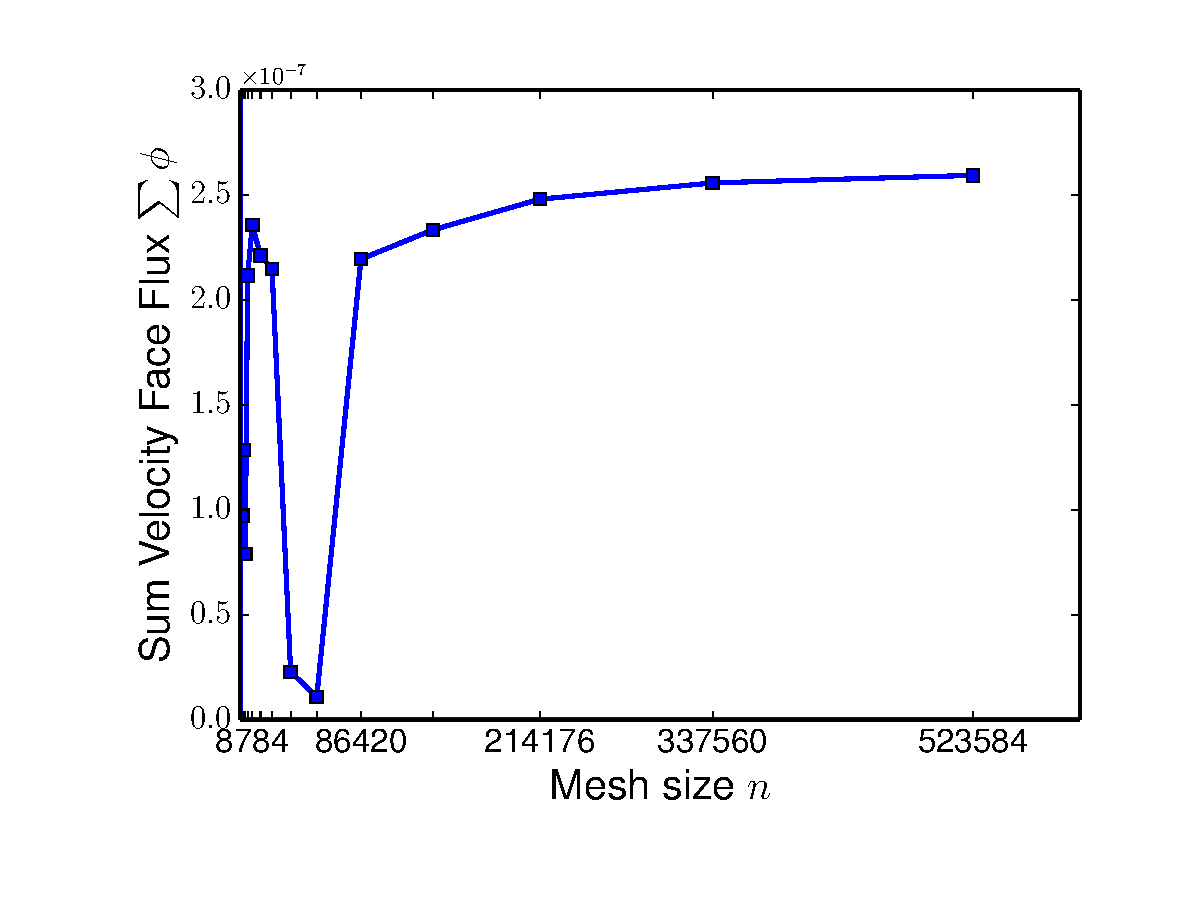
\includegraphics[width=0.79\textwidth]{fig12_Flux-end-20-times.pdf}
  \caption[Long-term behavior for different meshes]{
  \textbf{With a fixed choice of solver, boundary conditions, and initial conditions that lead to a stable convective state, we present the long-term behavior of the velocity face flux at the top slice for different meshes.}
    The face flux is reported as the average for the last 20 times saves for which the velocity flux is summed across a slice perpendicular to the loop, here we show the top slice.
    We choose a fixed time step of 0.005 for each simulation, and run the solver for 60 hours on 8 cores.
    The computational limit of mesh creation was a memory limit at 818280 cells, so we present results for meshes starting at 1600 cells and cells decreasing in size by a factor of 1.25 in both $y$ and $z$ up to a mesh of 523584 cells.
    For meshes with more than 80,000 cells we see that the solutions are very similar.
    The smaller meshes generate increasing unstable flow behavior, leading to oscillations of flux and then flow reversals for the smallest meshes of size 2500 and 1600 cells.
  }
  \label{fig:meshverification}
\end{figure}

\clearpage
\pagebreak
\subsection*{S2 Appendix: The Ehrhard and M\"{u}ller Equations}
\label{S2}

Following the derivation by Harris \cite{harris2011predicting}, itself a representation of the derivation of Gorman \cite{gorman1986} and namesakes Ehrhard and M\"{u}ller \cite{ehrhard1990dynamical}, we derive the equations governing a closed loop thermosyphon.

Similar to the derivation of the governing equations of computational fluid dynamics, we start with a small but finite volume inside the loop.
Here, however, the volume is described by $\pi r^2 R \text{d} \phi$ for $r$ the interior loop size (such that $\pi r^2$ is the area of a slice) and $R\text{d}\phi$ the arc length (width) of the slice.
Newton's second law states that momentum is conserved, such that the sum of the forces acting upon our finite volume is equal to the change in momentum of this volume.
Therefore we have the basic starting point for forces $\sum F$ and velocity $u$ as
\begin{equation} \sum F = \rho \pi r^2 R \text{d}\phi \diff{u}{t} .\end{equation}
The sum of the forces is $\sum F = F_{\{p,f,g\}}$ for net pressure, fluid shear, and gravity, respectively.
We write these as
\begin{align} & F_p = -\pi r^2 \text{d} \phi \pdiff{p}{\phi}\\
& F_w = -\rho \pi r^2 \text{d} \phi f_w\\
& F_g = -\rho \pi r^2 \text{d} \phi g \sin (\phi)\end{align}
where $\partial p /\partial \phi$ is the pressure gradient, $f_w$ is the wall friction force, and $g \sin (\phi)$ is the vertical component of gravity acting on the volume.

We now introduce the Boussinesq approximation which states that both variations in fluid density are linear in temperature $T$ and density variation is insignificant except when multiplied by gravity.
The consideration manifests as
\begin{equation*} \rho = \rho (T) \simeq \rho _\text{ref} (1 - \beta (T - T_\text{ref}) \end{equation*}
where $\rho _0$ is the reference density and $T_\text{ref}$ is the reference temperature, and $\beta$ is the thermal expansion coefficient.
The second consideration of the Boussinesq approximation allows us to replace $\rho$ with this $\rhoref$ in all terms except for $F_g$.
We now write momentum equation as
\begin{equation} -\pi r^2 \dphi \pdiff{p}{\phi} - \rhoref \phi r^2 R \dphi f_w
- \rhoref (1 - \rho (T- T_\text{ref}) ) \pi r^2 R \dphi g \sin (\phi) = \rhoref \pi r^2 R \dphi \diff{u}{t}. \end{equation}
Canceling the common $\pi r^2$, dividing by $R$, and pulling out $\dphi$ on the LHS we have
\begin{equation} -\dphi \left ( \pdiff{p}{\phi}  \frac{1}{R} - \rhoref f_w - \rhoref (1 - \rho (T- T_\text{ref}) ) g \sin (\phi) \right ) = \rhoref \dphi \diff{u}{t}. \label{eq:EM07} \end{equation}
We integrate this equation over $\phi$ to eliminate many of the terms, specifically we have
\begin{align*}
& \int _{0} ^{2\pi} -\dphi \pdiff{p}{\phi} \frac{1}{R} \rightarrow 0\\
& \int _{0} ^{2\pi} -\dphi \rhoref g \sin (\phi) \rightarrow 0\\
& \int _{0} ^{2\pi} -\dphi \rhoref \beta T_\text{ref} g \sin (\phi) \rightarrow 0.\end{align*}
Since $u$ (and hence $\diff{u}{\phi}$) and $f_w$ do not depend on $\phi$, we can pull these outside an integral over $\phi$ and therefore the momentum equation is now 
\begin{equation*} 2\pi f_w \rho _0 + \int _{0} ^{2\pi} \dphi \rhoref \beta T g \sin (\phi) = 2\pi \diff{u}{\phi} \rhoref .\end{equation*}
Diving out $2\pi$ and pull constants out of the integral we have our final form of the momentum equation
\begin{equation} f_w \rhoref + \frac{\rhoref \beta g }{2 \pi} \int _{0} ^{2\pi} \dphi T \sin (\phi) = \diff{u}{\phi} \rhoref \label{eq:EM10}.\end{equation}
Now considering the conservation of energy within the thermosyphon, the energy change within a finite volume must be balanced by transfer within the thermosyphon and to the walls.
The internal energy change is given by
\begin{equation} \rhoref \pi r^2 R \dphi \left ( \pdiff{T}{t} + \frac{u}{R}\pdiff{T}{\phi} \right ) \label{eq:EMeg1}\end{equation}
which must equal the energy transfer through the wall, which is, for $T_w$ the wall temperature:
\begin{equation} \dot{q} = -\pi r^2 R \dphi h_w (T - T_w) . \label{eq:EMeg2} \end{equation}
Combining Equations \ref{eq:EMeg1} and \ref{eq:EMeg2} (and canceling terms) we have the energy equation:
\begin{equation} \left ( \pdiff{T}{t} + \frac{u}{R}\pdiff{T}{\phi} \right ) = \frac{-h_w}{\rhoref c_p} \left( T - T_w \right ) \label{eq:EMeq}.\end{equation}
The $f_w$ which we have yet to define and $h_w$ are fluid-wall coefficients and can be described by \cite{ehrhard1990dynamical}:
\begin{align*} & h_w = h_{w_0} \left ( 1 + K h(|x_1|) \right ) \\
& f_w = \frac{1}{2} \rhoref f_{w_0} u .\end{align*}
We have introduced an additional function $h$ to describe the behavior of the dimensionless velocity $x_1 \alpha u$.
This function is defined piece-wise as 
\begin{equation} h (x) = \left \{ \begin{array}{ll} x^{1/3} & ~~\text{when} ~x \geq 1\\ p (x) & ~~\text{when} ~ x <1 \end{array} \right. \label{eq:h_defined} \end{equation} 
where $p(x)$ can be defined as $p(x) = \left( 44x^2 -55 x^3 + 20x^4 \right ) /9$ such that $p$ is analytic at 0 \cite{harris2011predicting}.

Taking the lowest modes of a Fourier expansion for $T$ for an approximate solution, we consider:
\begin{equation} T(\phi , t) = C_0 (t) + S(t) \sin (\phi ) + C(t) \cos (\phi) . \end{equation}
By substituting this form into Equations \ref{eq:EM10} and \ref{eq:EMeq} and integrating, we obtain a system of three equations for our solution.
We then follow the particular nondimensionalization choice of Harris \etal such that we obtain the following ODE system, which we refer to as the Ehrhard-M\"{u}ller equations:
\begin{align}
& \diff{x_1}{t'} = \alpha (x_2 - x_1),\\
& \diff{x_2}{t'} = \beta x_1 - x_2 (1 + Kh(|x_1|)) - x_1x_3,\\
& \diff{x_3}{t'} = x_1x_2 - x_3 (1 + Kh(|x_1|)) .\end{align}
The nondimensionalization is given by the change of variables
\begin{align}
& t' = \frac{h_{w_0}}{\rhoref c_p}t,\\
& x_1 = \frac{\rhoref c_p }{R h_{w_0}} u, \\
& x_2 = \frac{1}{2} \frac{\rhoref c_p \beta g}{ R h_{w_0} f_{w_0}} \Delta T_{3-9}, \\
& x_3 = \frac{1}{2} \frac{\rhoref c_p \beta g}{ R h_{w_0} f_{w_0}} \left ( \frac{4}{\pi} \Delta T_w - \Delta T_{6-12} \right ) 
\end{align}
and
\begin{align}
& \alpha = \frac{1}{2} R c_p f_{w_0} / h_{w_0} ,\\
& \gamma = \frac{2}{\pi} \frac{\rhoref c_p \beta g}{Rh_{w_0} f_{w_0}} \Delta T_w. \end{align}

Through careful consideration of these non-dimensional variable transformations we verify that $x_1$ is representative of the mean fluid velocity, $x_2$ of the temperature difference between the 3 and 9 o'clock positions on the thermosyphon, and $x_3$ the deviation from the vertical temperature profile in a conduction state \cite{harris2011predicting}.

\clearpage
\pagebreak
\subsection*{S3 Appendix: Data Assimiliation}
\label{S3}

The TLM is the model which advances an initial perturbation $\delta \mbx_{i}$ at timestep $i$ to a final perturbation $\delta \mbx_{i+1}$ at timestep $i+1$.
The dynamical system we are interested in, Lorenz '63, is given as a system of ODE's:
\[ \frac{d\mbx}{dt} = F(\mbx) .\]
We integrate this system using a numerical scheme of our choice (in the given examples we use a second-order Runge-Kutta method), to obtain a model $M$ discretized in time.
\[ \mbx(t) = M[ \mbx(t_0) ] .\]
Introducing a small perturbation $\mby$, we can approximate our model $M$ applied to $\mbx(t_0) + \mby(t_0)$ with a Taylor series around $\mbx(t_0)$:
\begin{align*} M[ \mbx(t_0) + \mby(t_0) ] &= M [ \mbx(t_0) ] + \frac{\partial M}{\partial \mbx} \mby(t_0) + O [ \mby(t_0) ^2 ]\\ &\approx \mbx(t) + \frac{\partial M}{\partial \mbx} \mby(t_0) .\end{align*}
We can then solve for the linear evolution of the small perturbation $\mby(t_0)$ as 
\begin{equation} \frac{d\mby }{dt } = \mathbf{J} \mby \label{eq:ODETLM} \end{equation}
where $\mathbf{J} = \partial F / \partial \mbx$ is the Jacobian of $F$.
We can solve the above system of linear ordinary differential equations using the same numerical scheme as we did for the nonlinear model.

One problem with solving the system of equations given by Equation \ref{eq:ODETLM} is that the Jacobian matrix of discretized code is not necessarily identical to the discretization of the Jacobian operator for the analytic system.
This is a problem because we need to have the TLM of our model $M$, which is the time-space discretization of the solution to $d\mbx/dt = F(\mbx)$.
We can apply our numerical method to the $d\mbx/dt = F(\mbx)$ to obtain $M$ explicitly, and then take the Jacobian of the result.
This method is, however, prohibitively costly, since Runge-Kutta methods are implicit.
It is therefore desirable to take the derivative of the numerical scheme directly, and apply this differentiated numerical scheme to the system of equations $F(\mbx)$ to obtain the TLM.
A schematic of this scenario is illustrated in Figure \ref{fig:TLMscheme}.
To that the derivative of numerical code for implementing the EKF on models larger than 3 dimensions (i.e. global weather models written in Fortan), automatic code differentiation is used \cite{autodiff1981}.

\begin{figure}[h]
  \centering
  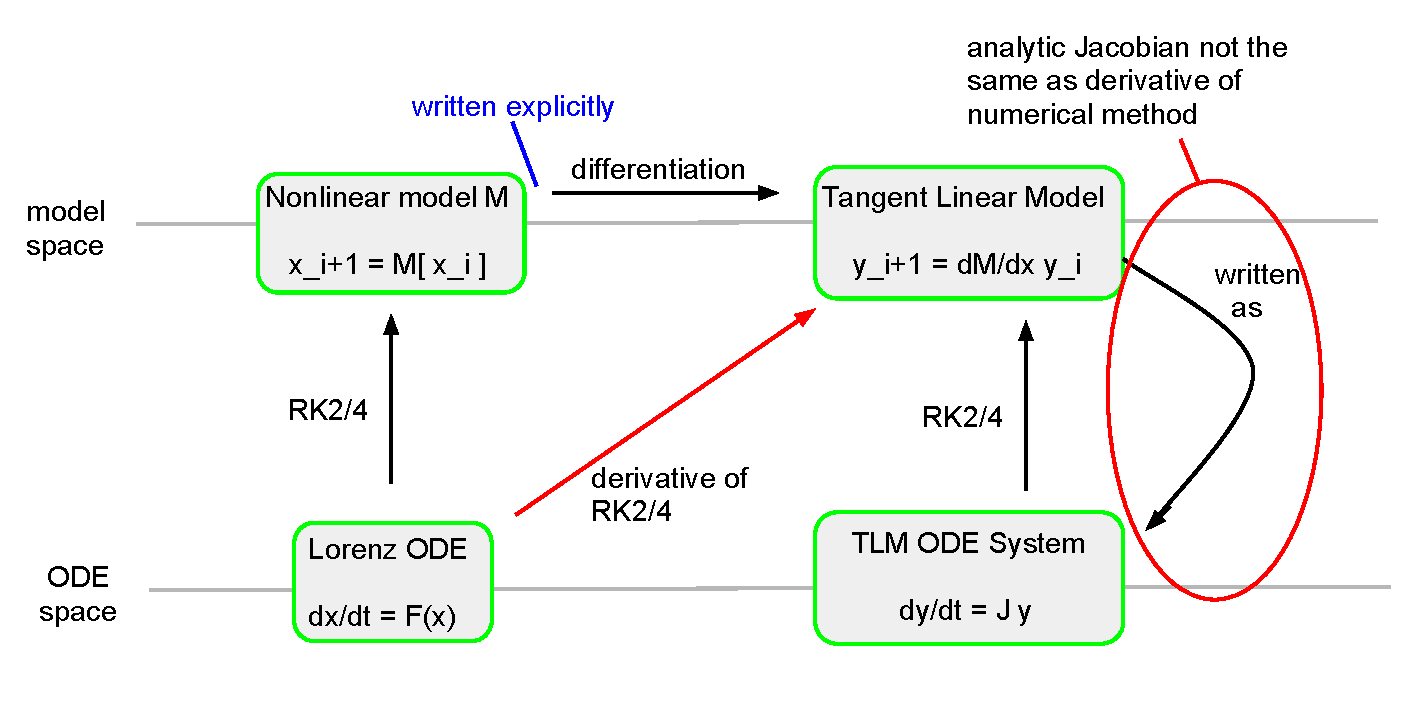
\includegraphics[width=0.89\textwidth]{fig13_TLM-explanation.pdf}
  \caption[An explanation of how and why the best way to obtain a TLM is with a differentiated numerical scheme]{
\textbf{    An explanation of how and why the best way to obtain a TLM is with a differentiated numerical scheme.
}    Both the Lorenz ODE and TLM ODE System can be solved by RK2/4, but the analytic Jacobian of TLM that would is not the same as the derivative of the numerical method.
    In particular, the derivative of the RK2/4 integrator is used to obtain a TLM that most accurately propogates error growth in the Lorenz '63 system.
  }
  \label{fig:TLMscheme}
\end{figure}

To verify our implementation of the TLM, we propagate a small error in the Lorenz '63 system and plot the difference between that error and the TLM predicted error, for each variable (Figure \ref{fig:TLMverification}).

\begin{figure}[h]
  \centering
  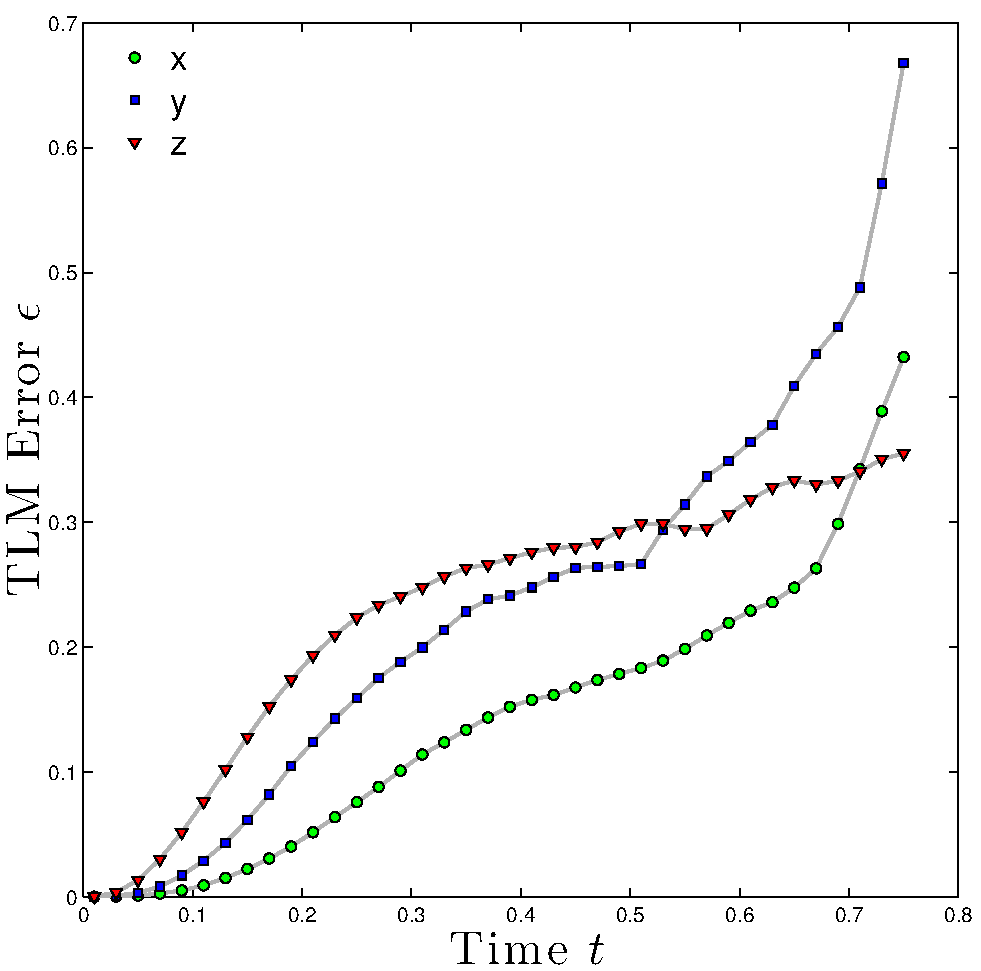
\includegraphics[width=0.45\textwidth]{fig14_TLM-verification003_noname.pdf}
  \caption[The future error predicted by the TLM is compared to the error growth in Lorenz '63 system for an initial perturbation with standard deviation of 0.1, averaged over 1000 TLM integrations]{
\textbf{    The future error predicted by the TLM is compared to the error growth in Lorenz '63 system for an initial perturbation with standard deviation of 0.1, averaged over 1000 TLM integrations.
}    The $\epsilon$ is not the error predicted by the TLM, but rather the error of the TLM in predicting the error growth.
    We see an intially linear error growth for small time, which is overcome by the nonlinearity of the Lorenz system for longer time.
  }
  \label{fig:TLMverification}
\end{figure}

With a finite ensemble size, the ensemble method is only an approximation and therefore in practice it often fails to capture the full spread of error.
To better capture the model variance, additive and multiplicative inflation factors are used to obtain a good estimate of the error covariance matrix (Data Assimilation Section).
The spread of ensemble members in the $x_1$ variable of the Lorenz model, as distance from the analysis, can be seen in Figure \ref{fig:EnKFhist}.

\begin{figure}[h]
  \centering
  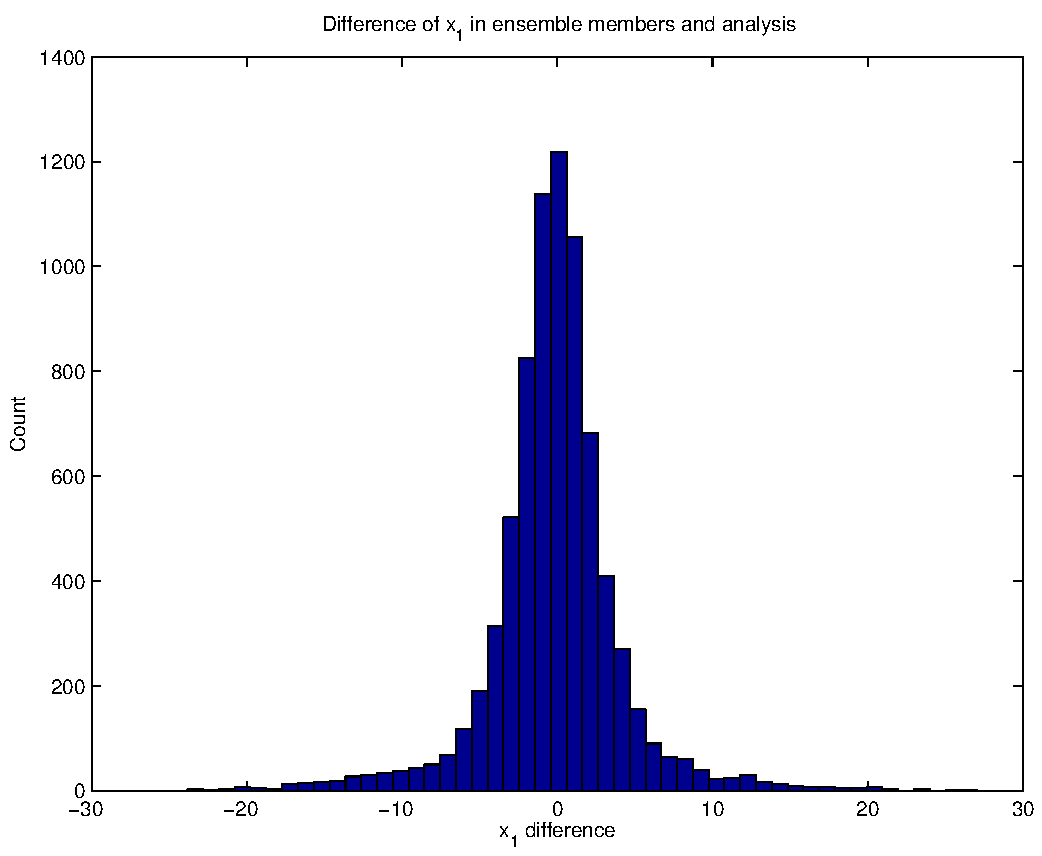
\includegraphics[width=0.79\textwidth]{fig15_EnKF-histogram-analysis.pdf}
  \caption[The difference of ensemble forecasts from the analysis is reported for 760 assimilation windows in one model run of length 200, with 10 ensemble members and an assimilation window of length 0.261]{
\textbf{    The difference of ensemble forecasts from the analysis is reported for 760 assimilation windows in one model run of length 200, with 10 ensemble members and an assimilation window of length 0.261.
}    This has the same shape of as the difference between ensemble forecasts and the mean of the forecasts (not shown).
    This spread of ensemble forecasts is what allows us to estimate the error covariance of the forecast model, and appears to be normally distributed.
  }
  \label{fig:EnKFhist}
\end{figure}

In computing the error covariance $\mbP_f$ from the ensemble, we wish to add up the error covariance of each forecast with respect to the mean forecast. 
But this would underestimate the error covariance, since the forecast we're comparing against is used in the ensemble average (to obtain the mean forecast).
Therefore, to compute the error covariance matrix for each forecast, that forecast itself is excluded from the ensemble average forecast.

We can see the classic spaghetti of the ensemble with this filter implemented on Lorenz 63 in Figure \ref{fig:spaghetti}.

\begin{figure}[h]
  \centering
  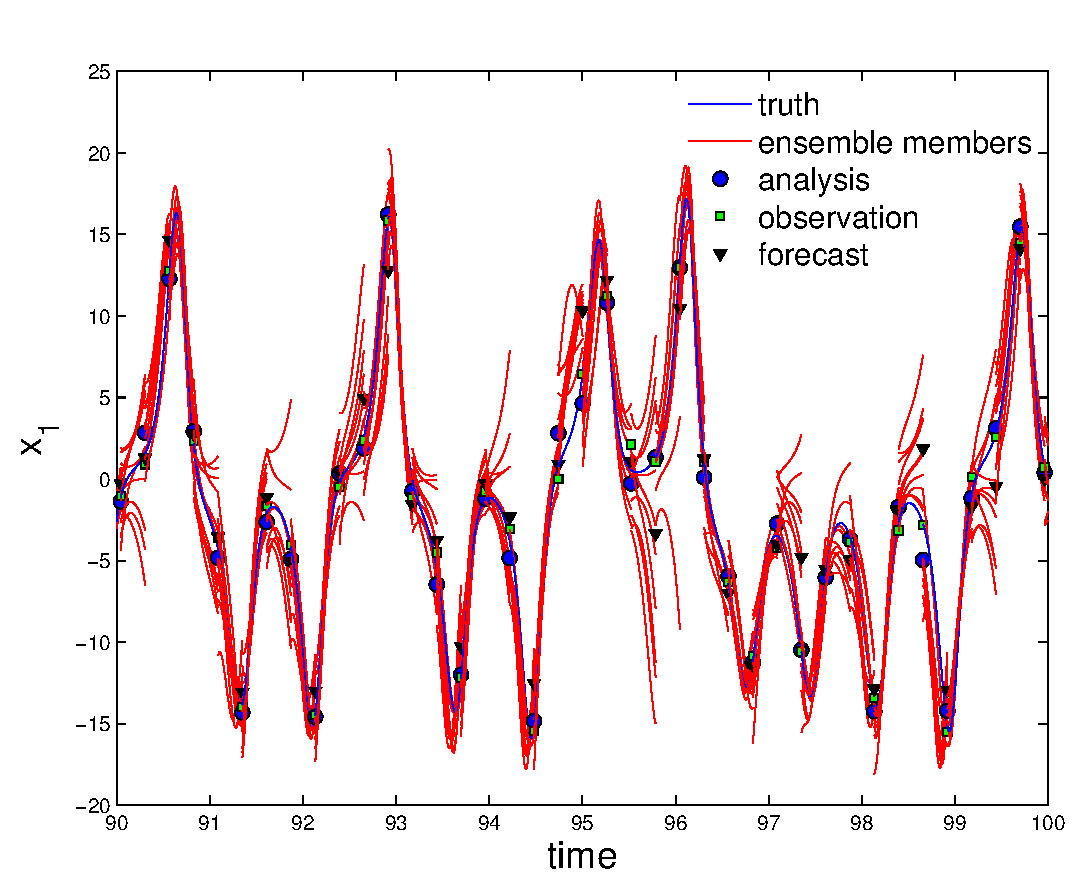
\includegraphics[width=0.99\textwidth]{fig16_EnKF_spaghetti.pdf}
  \caption[A sample time-series of the ensembles used in the EnKF]{
\textbf{    A sample time-series of the ensembles used in the EnKF.
}    In all tests, as seen here, 10 ensemble members are used.
    For this run, 384 assimilation cycles are performed with a window length of 0.26 model time units.
    We can see that the ensemble member state after assimilation better represents the uncertainty of the analysis state and enables some ensemble members to stay close to the true state.
  }
  \label{fig:spaghetti}
\end{figure}

We denote the forecast within an ensemble filter as the average of the individual ensemble forecasts, and an explanation for this choice is substantiated by Burgers \cite{burgers1998analysis}.
The general EnKF which we use is most similar to that of Burgers.
Many algorithms based on the EnKF have been proposed and include the Ensemble Transform Kalman Filter (ETKF) \cite{ott2004local}, Ensemble Analysis Filter (EAF) \cite{anderson2001new}, Ensemble Square Root Filter (EnSRF) \cite{tippett2003ensemble}, Local Ensemble Kalman Filter (LEKF) \cite{ott2004local}, and the Local Ensemble Transform Kalman Filter (LETKF) \cite{hunt2007efficient}.
A comprehensive overview through 2003 is provided by Evensen \cite{evensen2003ensemble}.
For further details on the most advanced methods, beyond what is provided in the body of the paper, we direct the reader the above references and the derivations provided in \cite{reagan2013}.

\clearpage
\pagebreak
\subsection*{S4 Appendix: Additional DMD Details}
\label{S4}

The general algorithm for DMD is provided in the Dynamic Mode Decomposition Section, and here we supply more results of the DMD procedure.
The timeseries from which we computed the decomposition is shown in Figure \ref{fig:DMD-timeseries}.

\begin{figure}[h]
  \centering
  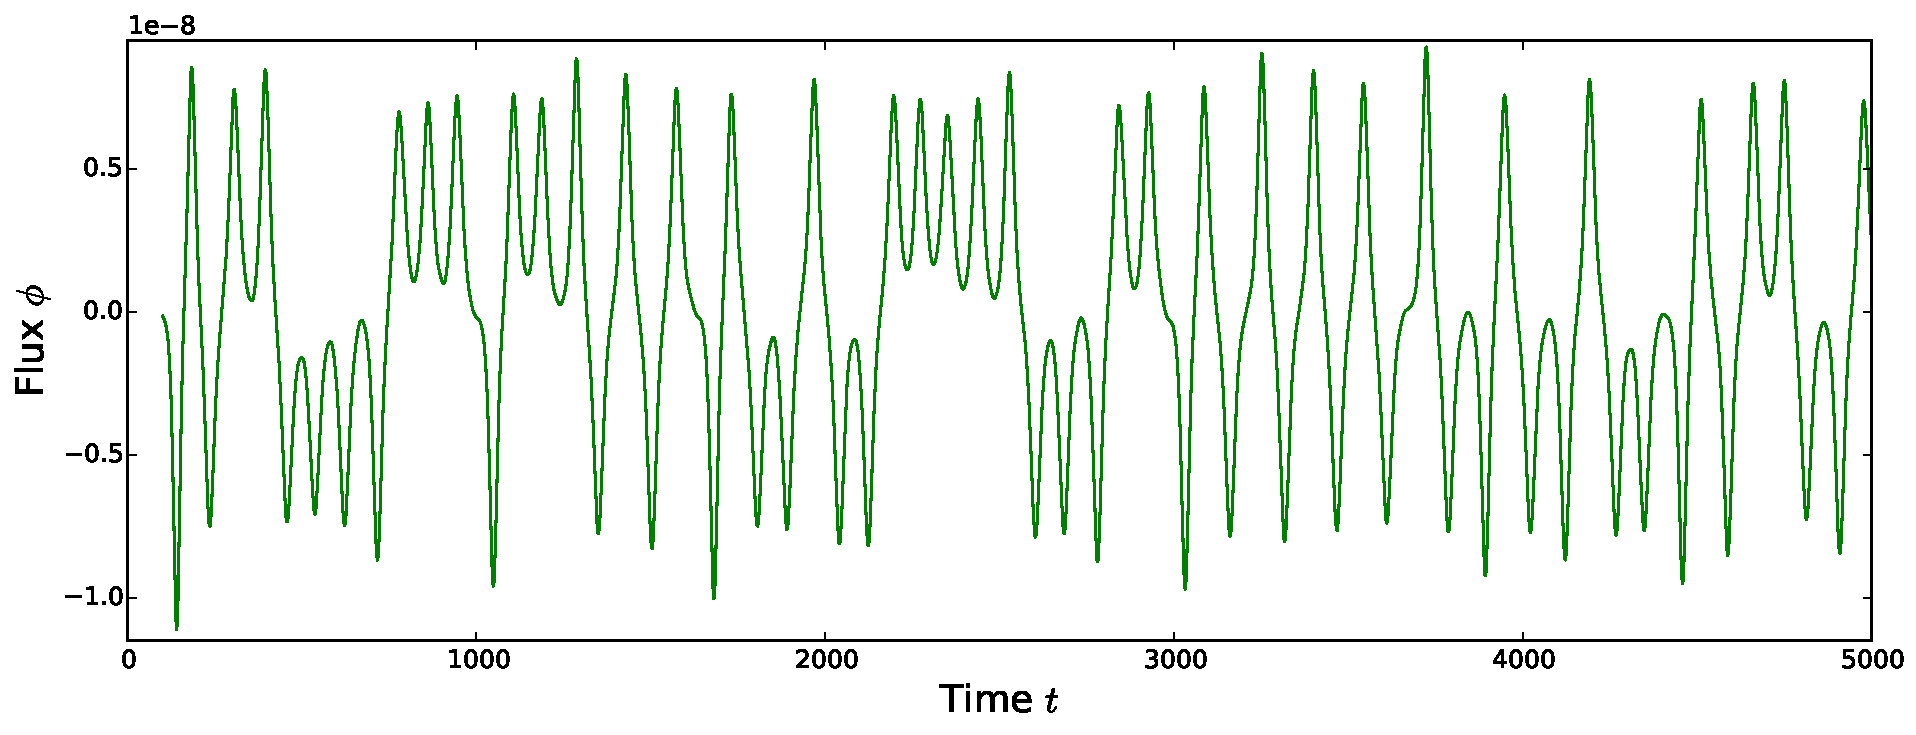
\includegraphics[width=0.98\textwidth]{fig17_DMD-data-timeseries-longer-wide.pdf}
  \caption[]{
\textbf{    Flux timeseries on which DMD is performed.
}    We report the flux as the sum of the face flux values on a slice of the loop at the 9 o'clock position.
    In this flux timeseries we see dynamics visually similar to the $x_1$ variable of the Lorenz 63 system.
    Residence time in either flow direction is aperiodic and unstable with the flow speed oscillating within a single direction with growing amplitude until reversing.
  }
  \label{fig:DMD-timeseries}  
\end{figure}

The real and imaginary components of the DMD eigenvalues are shown in both un-mapped and mapped form in Figure \ref{fig:DMD-eigenvalues}.

\begin{figure}[h]
  \centering
  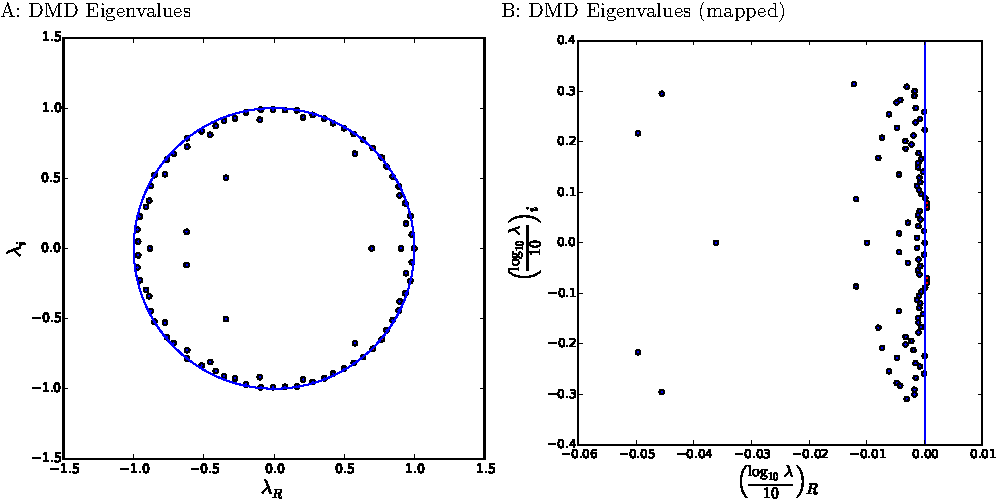
\includegraphics[width=0.98\textwidth]{fig18_eigenvalues-both-labeled.pdf}
  \caption[]{
\textbf{    Eigenvalues of DMD Modes presented in both raw and scaled (mapped) form.
}    In Panel A we see the eigenvalue of each DMD mode on the complex plane, with an inset unit circle.
    Those eigenvalues with magnitude greater than 1 are shown in red.
    In Panel B we see the same eigenvalues on the complex plane, transformed by the base 10 logarithm.
    Again we color in red those eigenvalues with real part greater than 0.
  }
  \label{fig:DMD-eigenvalues}  
\end{figure}

\clearpage
\pagebreak

\begin{thebibliography}{10}

\bibitem{weather-violence2013}
Hsiang SM, Burke M, Miguel E.
\newblock Quantifying the Influence of Climate on Human Conflict.
\newblock Science. 2013;341(6151).
\newblock Available from:
  \url{http://www.sciencemag.org/content/341/6151/1235367.abstract}.

\bibitem{ginsberg2008detecting}
Ginsberg J, Mohebbi MH, Patel RS, Brammer L, Smolinski MS, Brilliant L.
\newblock Detecting influenza epidemics using search engine query data.
\newblock Nature. 2008;457(7232):1012--1014.

\bibitem{sornette2006predictability}
Sornette D, Zhou WX.
\newblock Predictability of large future changes in major financial indices.
\newblock International Journal of Forecasting. 2006;22(1):153--168.

\bibitem{asur2010predicting}
Asur S, Huberman BA.
\newblock Predicting the future with social media.
\newblock In: Web Intelligence and Intelligent Agent Technology (WI-IAT), 2010
  IEEE/WIC/ACM International Conference on. vol.~1. IEEE; 2010. p. 492--499.

\bibitem{savely1972}
Savely R, Cockrell B, , Pines S.
\newblock Apollo Experience Report - Onboard Navigational and Alignment
  Software.
\newblock Technical Report. 1972;.

\bibitem{bauer2015quiet}
Bauer P, Thorpe A, Brunet G.
\newblock The quiet revolution of numerical weather prediction.
\newblock Nature. 2015;525(7567):47--55.

\bibitem{yang2006}
Yang SC, Baker D, Li H, Cordes K, Huff M, Nagpal G, et~al.
\newblock Data Assimilation as Synchronization of Truth and Model: Experiments
  with the Three-Variable Lorenz System*.
\newblock Journal of the atmospheric sciences. 2006;63(9):2340--2354.

\bibitem{harris2011predicting}
Harris KD, Ridouane EH, Hitt DL, Danforth CM.
\newblock Predicting flow reversals in chaotic natural convection using data
  assimilation.
\newblock arXiv preprint arXiv:11085685. 2011;.

\bibitem{keller1966}
Keller JB.
\newblock Periodic oscillations in a model of thermal convection.
\newblock J Fluid Mech. 1966;26(3):599--606.

\bibitem{welander1967}
Welander P.
\newblock On the oscillatory instability of a differentially heated fluid loop.
\newblock International Geophysics Series. 1995;59.

\bibitem{creveling1975stability}
Creveling H, PAZ D, Baladi J, Schoenhals R.
\newblock Stability characteristics of a single-phase free convection loop.
\newblock Journal of Fluid Mechanics. 1975;67(part 1):65--84.

\bibitem{gorman1984}
Gorman M, Widmann P.
\newblock Chaotic flow regimes in a convection loop.
\newblock Phys Rev Lett. 1984;(52):2241--2244.

\bibitem{gorman1986}
Gorman M, Widmann P, Robbins K.
\newblock Nonlinear dynamics of a convection loop: a quantitative comparison of
  experiment with theory.
\newblock Physica D. 1986;(19):255--267.

\bibitem{ehrhard1990dynamical}
Ehrhard P, M{\"u}ller U.
\newblock Dynamical behaviour of natural convection in a single-phase loop.
\newblock Journal of Fluid mechanics. 1990;217:487--518.

\bibitem{yuen1999}
Yuen P, Bau H.
\newblock Optimal and adaptive control of chaotic convection.
\newblock Phys Fluids. 1999;(11):1435--1448.

\bibitem{jiang2003}
Jiang Y, Shoji M.
\newblock Spatial and temporal stabilities of flow in a natural circulation
  loop: influences of thermal boundary condition.
\newblock J Heat Trans. 2003;(125):612--623.

\bibitem{burroughs2005reduced}
Burroughs E, Coutsias E, Romero L.
\newblock A reduced-order partial differential equation model for the flow in a
  thermosyphon.
\newblock Journal of Fluid Mechanics. 2005;543:203--238.

\bibitem{desrayaud2006numerical}
Desrayaud G, Fichera A, Marcoux M.
\newblock Numerical investigation of natural circulation in a 2D-annular
  closed-loop thermosyphon.
\newblock International journal of heat and fluid flow. 2006;27(1):154--166.

\bibitem{ridouane2010}
Ridouane EH, Danforth CM, Hitt DL.
\newblock A 2-D numerical study of chaotic flow in a natural convection loop.
\newblock International Journal of Heat and Mass Transfer. 2010;53(1):76--84.

\bibitem{louisos2013}
Louisos WF, Hitt DL, Danforth CM.
\newblock Chaotic flow in a 2D natural convection loop with heat flux
  boundaries.
\newblock International Journal of Heat and Mass Transfer. 2013;61:565--576.

\bibitem{glenn2013}
Glenn D.
\newblock Characterizing weather in a thermosyphon: an atmosphere that hangs on
  a wall; 2013.
\newblock Undergraduate Honors Thesis, University of Vermont.

\bibitem{jasak2007}
Jasak H, Jemcov A, Tukovic Z.
\newblock OpenFOAM: A C++ library for complex physics simulations.
\newblock In: International Workshop on Coupled Methods in Numerical Dynamics,
  IUC, Dubrovnik, Croatia; 2007. p. 1--20.

\bibitem{issa1986solution}
Issa RI.
\newblock Solution of the implicitly discretised fluid flow equations by
  operator-splitting.
\newblock Journal of Computational physics. 1986;62(1):40--65.

\bibitem{lorenc1986analysis}
Lorenc AC.
\newblock Analysis methods for numerical weather prediction.
\newblock Quarterly Journal of the Royal Meteorological Society.
  1986;112(474):1177--1194.

\bibitem{kalnay2003}
Kalnay E.
\newblock Atmospheric modeling, data assimilation, and predictability.
\newblock Cambridge university press; 2003.

\bibitem{danforth2007estimating}
Danforth CM, Kalnay E, Miyoshi T.
\newblock Estimating and correcting global weather model error.
\newblock Monthly weather review. 2007;135(2):281--299.

\bibitem{li2009accounting}
Li H, Kalnay E, Miyoshi T, Danforth CM.
\newblock Accounting for model errors in ensemble data assimilation.
\newblock Monthly Weather Review. 2009;137(10):3407--3419.

\bibitem{danforth2008using}
Danforth CM, Kalnay E.
\newblock Using singular value decomposition to parameterize state-dependent
  model errors.
\newblock Journal of the Atmospheric Sciences. 2008;65(4):1467--1478.

\bibitem{bishop2001adaptive}
Bishop CH, Etherton BJ, Majumdar SJ.
\newblock Adaptive sampling with the ensemble transform Kalman filter. Part I:
  Theoretical aspects.
\newblock Monthly weather review. 2001;129(3):420--436.

\bibitem{kalnay2007a}
Kalnay E, Li H, Miyoshi T, Yang SC, Ballabrera-Poy J.
\newblock 4-D-Var or ensemble Kalman filter?
\newblock Tellus A. 2007;59(5):758--773.

\bibitem{ott2004local}
Ott E, Hunt BR, Szunyogh I, Zimin AV, Kostelich EJ, Corazza M, et~al.
\newblock A local ensemble Kalman filter for atmospheric data assimilation.
\newblock Tellus A. 2004;56(5):415--428.

\bibitem{hunt2007efficient}
Hunt BR, Kostelich EJ, Szunyogh I.
\newblock Efficient data assimilation for spatiotemporal chaos: A local
  ensemble transform Kalman filter.
\newblock Physica D: Nonlinear Phenomena. 2007;230(1):112--126.

\bibitem{tu2013dynamic}
Tu JH, Rowley CW, Luchtenburg DM, Brunton SL, Kutz JN.
\newblock On dynamic mode decomposition: theory and applications.
\newblock arXiv preprint arXiv:13120041. 2013;.

\bibitem{bishop2011a}
Bishop CH, Hodyss D.
\newblock Adaptive Ensemble Covariance Localization in Ensemble 4D-VAR State
  Estimation.
\newblock Monthly Weather Review. 2011 April;139(4):7.

\bibitem{reagan2013}
Reagan A.
\newblock Predicting Flow Reversals in a Computational Fluid Dynamics Simulated
  Thermosyphon using Data Assimilation.
\newblock arXiv:13122142. 2013;.

\bibitem{patankar1972calculation}
Patankar SV, Spalding DB.
\newblock A calculation procedure for heat, mass and momentum transfer in
  three-dimensional parabolic flows.
\newblock International Journal of Heat and Mass Transfer.
  1972;15(10):1787--1806.

\bibitem{ferziger1996computational}
Ferziger JH, Peri{\'c} M.
\newblock Computational methods for fluid dynamics. vol.~3.
\newblock Springer Berlin; 1996.

\bibitem{autodiff1981}
Rall LB.
\newblock Automatic Differentiation: Techniques and Applications (Lecture Notes
  in Computer Science).
\newblock Springer; 1981.

\bibitem{burgers1998analysis}
Burgers G, Jan~van Leeuwen P, Evensen G.
\newblock Analysis scheme in the ensemble Kalman filter.
\newblock Monthly weather review. 1998;126(6):1719--1724.

\bibitem{anderson2001new}
Anderson MJ.
\newblock A new method for non-parametric multivariate analysis of variance.
\newblock Austral Ecology. 2001;26(1):32--46.

\bibitem{tippett2003ensemble}
Tippett MK, Anderson JL, Bishop CH, Hamill TM, Whitaker JS.
\newblock Ensemble square root filters*.
\newblock Monthly Weather Review. 2003;131(7):1485--1490.

\bibitem{evensen2003ensemble}
Evensen G.
\newblock The ensemble Kalman filter: Theoretical formulation and practical
  implementation.
\newblock Ocean dynamics. 2003;53(4):343--367.

\end{thebibliography}













\end{document}
